Betrachtet werden Funktionen, welche beide 9600 Samples lang und in Abbildung \ref{deconvolve:1d} dargestellt sind.
Die zwei Kurven wurden mit einer diskreten Wavelet-Transformation mit 13 Level analysiert.
Dabei wurde das Haar-Wavelet verwendet.

Kann nun ein Zusammenhang zwischen den Wavelet-koeffizienten erkannt werden?
Die Hoffnung war es, diesen Zusammenhang in als Funktion zu formulieren um dann die Koeffizienten von $f(x)$ hier $cf_k$ genannt, soweit zu manipulieren, bis sie den Koeffizienten von $g(x)$, analog $cg_k$, genug ähnlich sind.
Der Index $k$ soll dabei das entsprechende Level der Koeffizienten sein.
\begin{figure}[h]
\centering
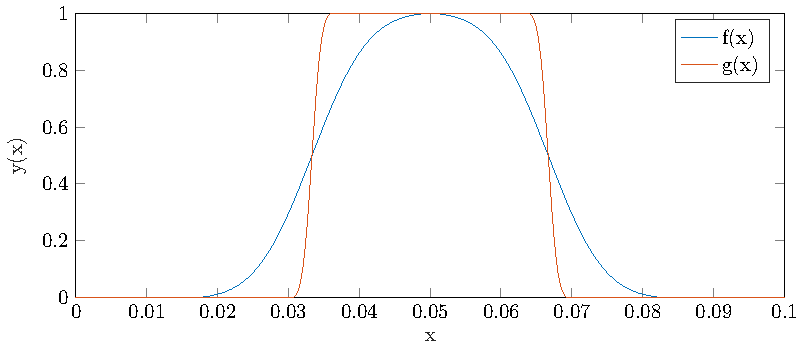
\includegraphics[width=0.9\textwidth]{./papers/deconvolve/pictures/1d.pdf}
\caption{Funktion\label{deconvolve:1d}}
\end{figure}
Die Rücktransformation mit den manipulierten $cf_k$ sollte dann eine Funktion liefern, welche $g(x)$ nahe kommt.
Bei Erfolg hätte man also eine Funktion erarbeitet, welche aus der unscharfen $f(x)$ eine etwas schärfere Funktion $g(x)$ macht. 

\subsection{Koeffizienten manipulieren}
Auf Level 1 sind die Koeffizienten mit der höchsten Auflösung, Level 13 demnach die gröbsten.
Abbildung \ref{deconvolve:level1} zeigt die Koeffizienten des ersten Levels der Funktionen $f(x)$ und $g(x)$.
\begin{figure}[h]
\centering
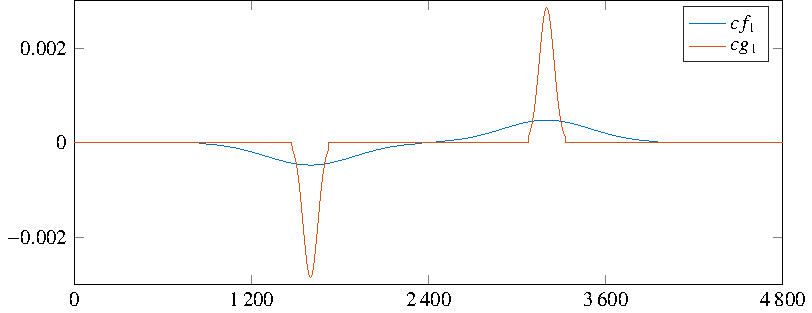
\includegraphics[width=0.9\textwidth]{./papers/deconvolve/pictures/level/level1.pdf}
\caption{Level 1 unverändert\label{deconvolve:level1}}
\end{figure}
Nun wird mit einer geeigneten Funktion versucht, die blaue Kurve anzupassen bis sie der orangen Kurve möglichst ähnlich ist. Man erkennt klar, dass die $cf_1$ unter einer gewissen Schwelle abgeschwächt und darüber überproportional verstärtk werden müssen. Dafür scheint sich
\begin{align}
m\cdot \left(\frac{|cf_k|}{m}\right)^{\alpha}\cdot \frac{|cf_k|}{cf_k}, \qquad m,\alpha\in\mathbb{R}
\label{deconvolve:funktion}
\end{align}
als Beziehung zwischen den \glqq unscharfen\grqq{} und \glqq scharfen\grqq{} Koeffizienten anzubieten.
In \eqref{deconvolve:funktion} stehen uns zwei Freiheitsgrade zur Verfügung.
Mit dem Parameter $\alpha$ wird die Verstärkung bestimmt, währenddessen $m$ die Schwelle festhält.
Der letzte Faktor wird nur zur Erhaltung des Vorzeichens gebraucht.
Für $m$ kann also genau der Schnittpunkt zwischen den beiden Kurven gewählt werden.
$\alpha$ wird dann so bestimmt, dass die beiden Spitzen auseinanderfallen.
\begin{figure}[h]
\centering
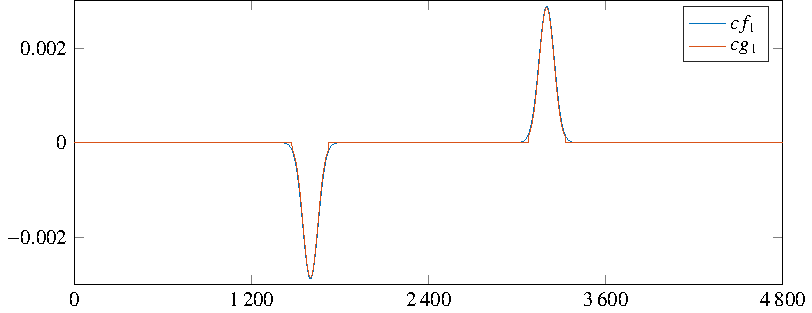
\includegraphics[width=0.9\textwidth]{./papers/deconvolve/pictures/level/level1_n.pdf}
\caption{Level 1 mit veränderten $cf_1$\label{deconvolve:level1_n}}
\end{figure}
Abbildung \ref{deconvolve:level1_n} zeigt die Beziehung \eqref{deconvolve:funktion} wiederum auf das erste Level angewendet. Der unterschied zwischen den beiden Kurven ist nur noch schwach erkennbar.

\subsection{Koeffizienten auf höheren Level}
Die selbe Funktion \eqref{deconvolve:funktion} kann nun auch auf die anderen Level mit entsprechenden $m$ und $\alpha$ angewendet werden.
Abbildung \ref{deconvolve:level5} zeigt Level 5 vor und nach der Koeffizientenmanipulation.
\begin{figure}[h]
\centering
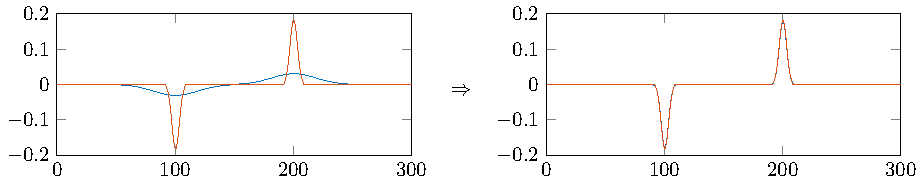
\includegraphics[width=0.9\textwidth]{./papers/deconvolve/pictures/level/level5.pdf}
\caption{Level 5 vorher und nachher\label{deconvolve:level5}}
\end{figure}
Auf diesem Level scheint alles noch wie erwünscht zu funktionieren.
Jedes Level höher kommen aber erwartungsgemäss weniger (halb so viele) Koeffizienten dazu.
Waren es im ersten noch 4800 sind es nun im fünften nur noch 300.
Auf dem Level 13 sind es dann nur noch zwei.
Deswegen wird es immer schwerer, die beiden Freiheitsgrade $m$ und $\alpha$ so zu wählen, dass noch eine Annäherung von $cf_k$ an $cg_k$ resultiert. Mit dieser Beispielfunktion $f(x)$ war es möglich mit der Beziehung \eqref{deconvolve:funktion} bis auf das Level 12 eine Verbesserung zu erreichen.

\subsection{Ergebnis}
Mit den nun angepassten Koeffizienten $cf_k$ sollte die Rücktransformation nun eine Funktion liefern, die sich in Richtung $g(x)$ bewegt hat.
In Abbildung \ref{deconvolve:result_1d} wird die Veränderung klar ersichtlich.
Verglichen mit der ursprünglichen Kurve $f_1(x)$ ist $f_2(x)$ deutlich näher an $g(x)$ gerückt, allerdings mit zusätzlichen Schwingungen.
\begin{figure}[h]
\centering
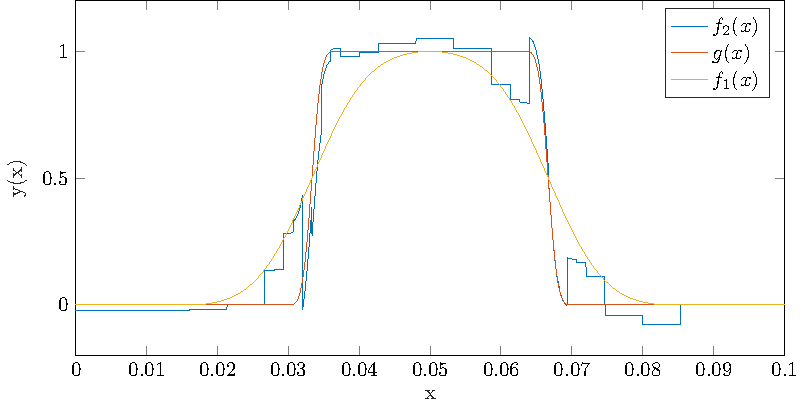
\includegraphics[width=0.9\textwidth]{./papers/deconvolve/pictures/result_1d.pdf}
\caption{Rücktransformation\label{deconvolve:result_1d}}
\end{figure}
